%!TEX root = ../ausarbeitung.tex
\section{Implementation}
\label{sec_implementation}

We implemented BugTracker as commandline-based Python tool.
It takes an image as input, and produces an RDF file with annotations of the found insects.
Template

\subsection{Contour Detection}
As a basic approach, we use Contour Detection to find insects in a given image.
The input image converted to gray-scale is used to detect edges as mentioned in Section \ref{sec_concepts}.
We use an adaptive threshold to create a binary image, which is then transformed by a morphological operation from OpenCV, in order to close gaps in areas of interest.
On this transformed binary image, an OpenCV contour detection function is applied, which groups connected edges into one contour (Figure \ref{fig:thresh}).
Those contours are a first approach on finding something on an image.
However, the threshold and edge detection algorithm can not possibly know, what we are looking for.
The found contours can be anything that appears to stand out from the background, not only insects.
This method is a good approach to just find anything on the image, but not precise enough for our needs.
\begin{center}
	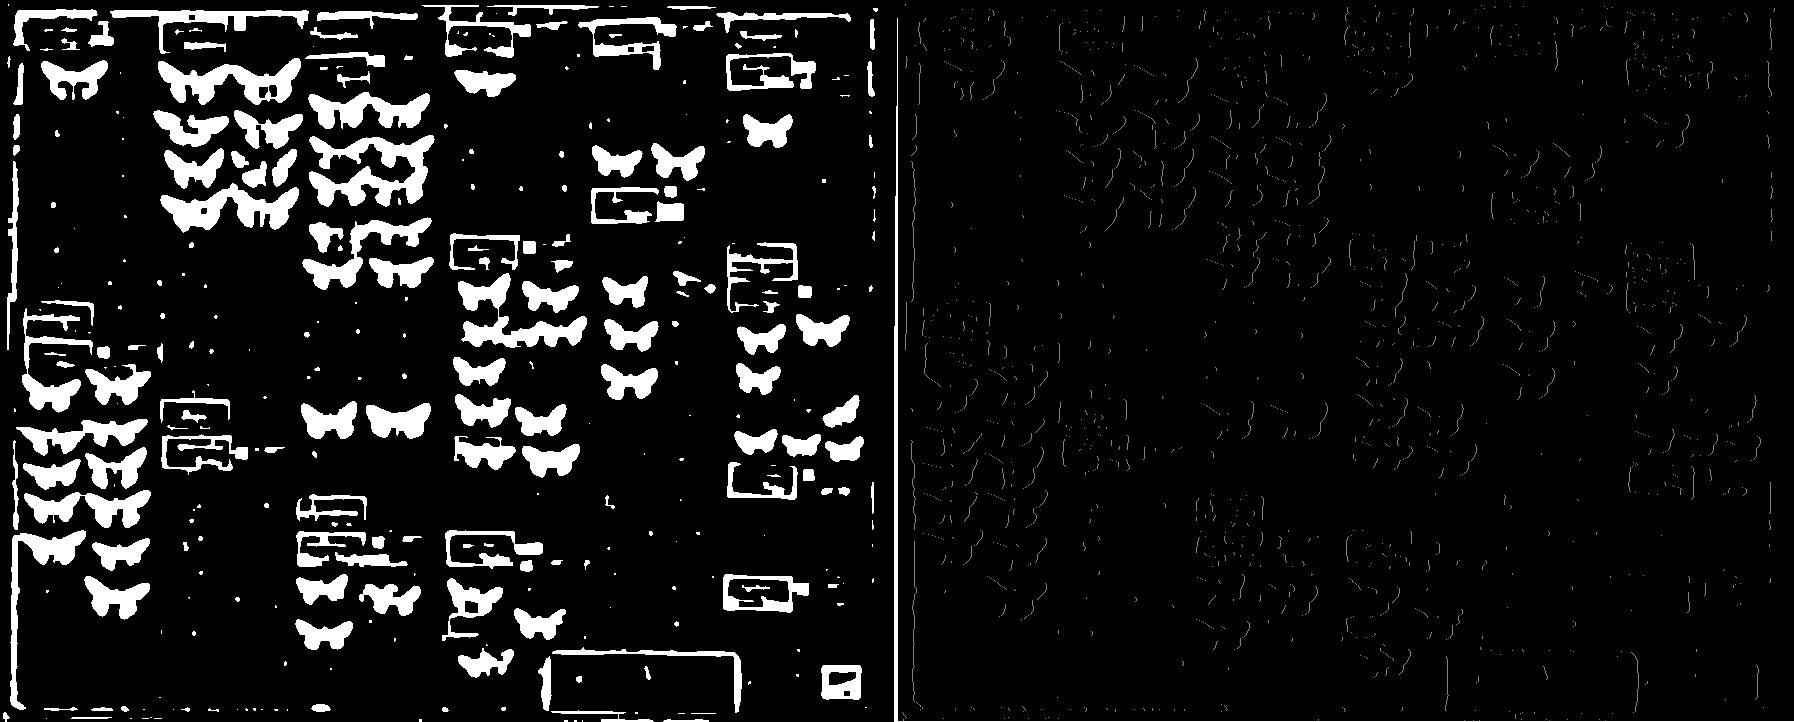
\includegraphics[width=1.0\textwidth]{images/chap5_thresh.png}
	\captionof{figure}{Binary image after using an adaptive threshold and morphological closing (left).
		Contour image created from binary image (right).}
	\label{fig:thresh}
\end{center}


\subsection{Template Matching}
To provide the algorithm an imagination of how the shapes which it is supposed to find look like, it is necessary to give it a sample shape to be geared on.
A possibility for that is using a template matching algorithm.
OpenCV provides this functionality, so the only thing to do was to define a comparison function.
By testing it turned out that CCOEFF gave the best results.
As templates cropped images from the insect library were used like in Figure \ref{fig:hesp_tmp}.
\begin{center}
	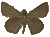
\includegraphics[width=0.1\textwidth]{images/hesp_template.jpg}
	\captionof{figure}{A template for butterflies}
	\label{fig:hesp_tmp}
\end{center}
The result of that OpenCV algorithm was a list of all sub-images with their corresponding match values describing how good they match the template.
The part of the image where we took the template from, of course always had a value of 1, which is the best possible value.
All other values are between -1 and 1, where a higher value means, that it matches the template better.
The next step is to set a threshold, defining from which value on sub-images are taken as matching.
A threshold of 0.41 worked best for us to avoid too many false positives and true negatives.

Using this algorithm a result like in Figure \ref{fig:no_frame_group} is generated.
\begin{center}
	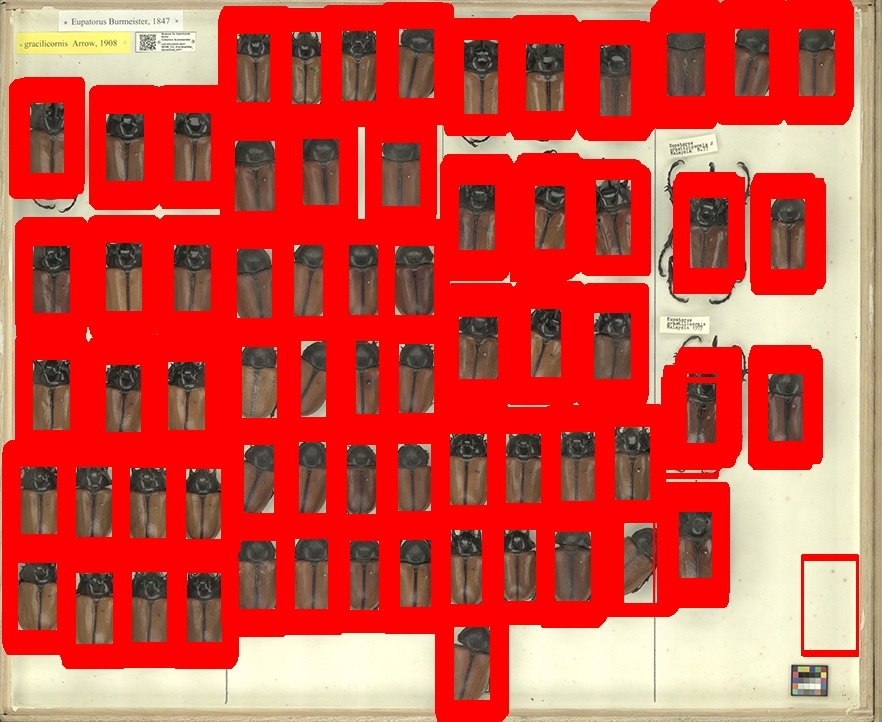
\includegraphics[width=0.8\textwidth]{images/no_frame_group.jpg}
	\captionof{figure}{Multiple matches per insect}
	\label{fig:no_frame_group}
\end{center}

As you can see the wide borders of the frames are the result of multiple overlapping matches, that are showing the same insect.
To group such corresponding matches together to one match, an overlay threshold of 30\% was defined to tell the algorithm when two frames are put together.
The same image as in Figure \ref{fig:no_frame_group} now with frame grouping in Figure \ref{fig:with_frame_group}
\begin{center}
	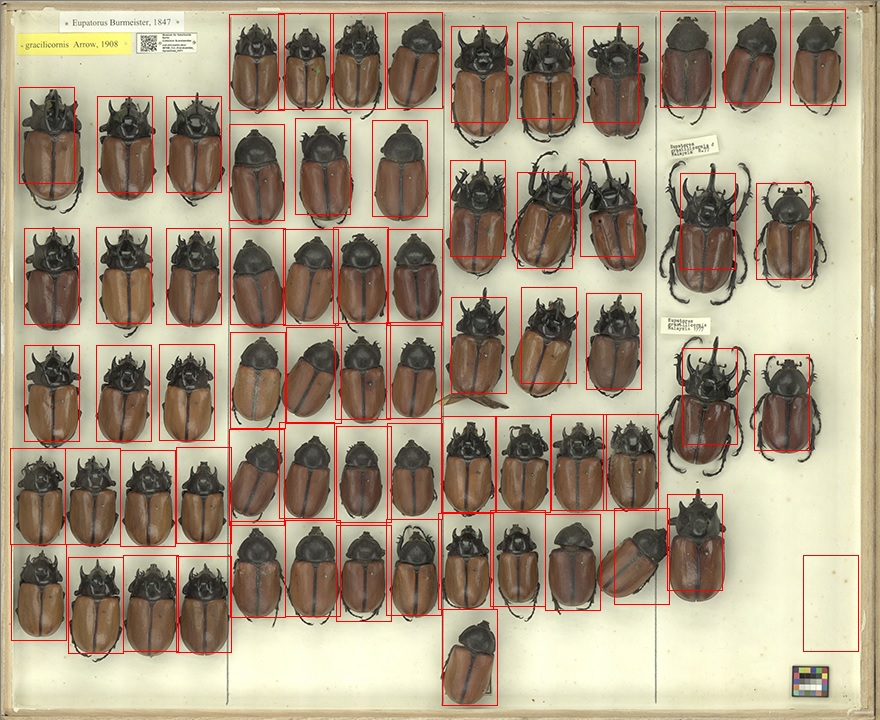
\includegraphics[width=0.8\textwidth]{images/with_frame_group.jpg}
	\captionof{figure}{Only one frame per insect after grouping corresponding ones together}
	\label{fig:with_frame_group}
\end{center}

In Figure \ref{fig:with_frame_group} you can see the results with the given algorithms so far.
As you can see there are many false positives left, which have to be discarded.
This is done by a second comparison using Histogram of Oriented Gradients.
If the matching value is below 0.95, the result is discarded.
Another problem is dirt and other unexpected noise on the image, that sometimes matches the template pretty well as a false positive.
An example for that is the false positive in Figure \ref{fig:with_frame_group} on the bottom right.
The soft shadow in the background describes a shape almost like one of the bugs.
To get rid of those results, the histogram of the whole image is generated to get the background color.
All matches now have to have an average color that has a certain difference to the background color to be taken as a match.
A final result can be seen in Figure \ref{fig:final_frames}.
\begin{center}
	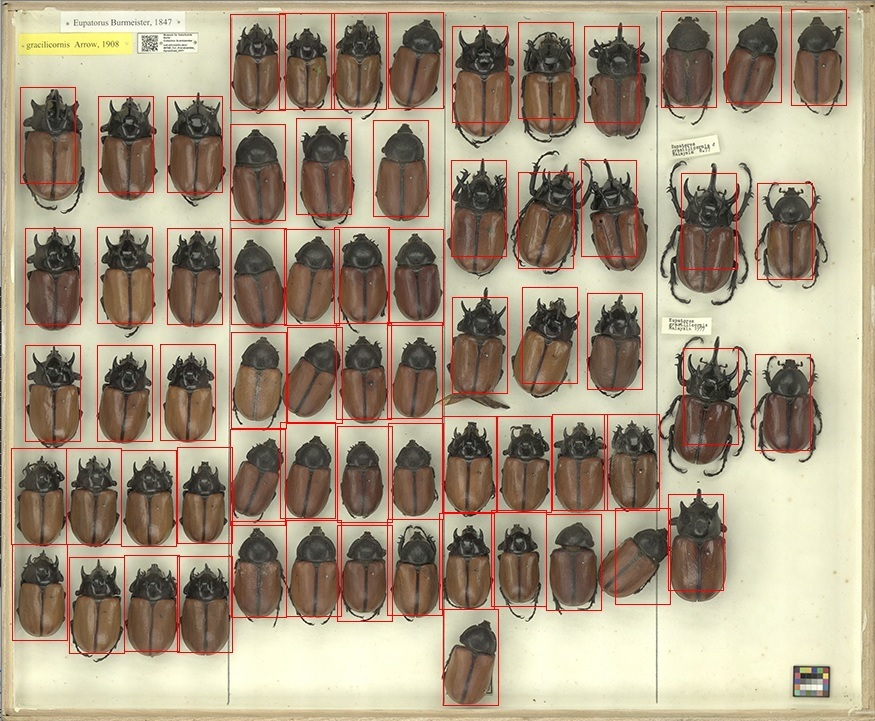
\includegraphics[width=0.8\textwidth]{images/final_frames.jpg}
	\captionof{figure}{The bottom right frame has gone by analyzing the histogram}
	\label{fig:final_frames}
\end{center}

\subsection{Automated Template Extraction}
Until this point, the templates were provided manually by cropping images. 
Since the annotation has to run fully automated, the template extraction also has to be done by the algorithm.
The Edge Detection algorithm is reused here to provide a list of potential templates.
This list is still full of false positives that have to be discarded.
In multiple steps, the following contours are thrown away: 
\begin{enumerate}
	\item Very small contours, that consist of less than 50 points.
	\item Contours that appear to be a label, if identified correctly.
	This is done by a template matching against some sample labels which were manually cropped out.
	Since labels look quite similar in each image, there is a chance that with this step those contours are discarded.
	\item 5\% of the number of contours are removed which have the highest height, 5\% which have the lowest height, 5\% that have the highest width, and 5\% that have the lowest width.
	This removes contours that have caught for example noise on the side of an image, which resembles e.g. the edge of the insect box (very long but thin contour).
	\item Contours with an extreme small or big area.
\end{enumerate}
After these steps, we have reduced the number of found contours that are potential templates for our Template Matching.
From the current set of potential templates, we extract one, which is representative for the insect species in that image.
This is done by apply template matching to all of our potential templates against each other.
The method \emph{matchTemplate} provided by OpenCV yields a score when matching a template against another image.
The higher the score, the better the match.
When matching each potential template against each other, we sum up the scores that are yielded, so that in the end the potential template with the highest score is our actual extracted template.
This of course has the premise, that after reducing the set of potential templates, there are more candidates which are actual insects, than other stuff, like labels, or just dirt on the box.
That is most of the time the case, but to not completely rely on that premise, we add multiple previously cropped out samples to the template matching process to improve the score of the templates that are actual insects.
We also add negative samples, such as labels, which reduce the score of unwanted templates.
After this process, we choose the potential template with the highest match score as our extracted template for our Template Matching step.

\subsection{Annotations}
The simplest annotation is just an RDF-triple locating a bug on an image and describing it as an organism. 
The definition for an organism and all properties we use to describe are part of the \emph{Darwin Core} \footnote{http://rs.tdwg.org/dwc/} Standard of describing living organisms.

We can extract further information from a CSV file that was provided by the \emph{Museum für Naturkunde} in Berlin.
It contains a general overview of all species in a photograph.
This includes dates and information about the family.

Whenever a new bug is found, it is added to the collection of bugs that will be written as RDF file at the end.
It is possible to annotate every bug with additional, specific properties.

Such information can be found in QR codes as described in the following section.

\subsubsection{QR Code Analysis}
Typically, each image contains multiple insect boxes with their own QR code that encodes a species specific URI.
We can link this URI to further information, which is basically the taxonomic classification of a bug, such as a its order, genus, and species.

To search QR codes in the images, we use the \emph{ZBar} library \footnote{http://zbar.sourceforge.net/}.
This Python library allows to obtain various bar codes from images and supports multiple types of bar codes.
It is also used by the \emph{Inselect} project to search and decode QR codes.
\emph{ZBar} locates and decodes QR codes, which returns the species URI in our case.

Once we have this URI, we can lookup the associated taxonomic data from a CSV file provided by the \emph{Museum für Naturkunde}.

The mapping from a found bug to its QR code proved to be more difficult than expected because of varying box layouts.
As there was no algorithm that matched everything correctly, we alternated the annotation approach to specify the taxonomic information that is common to all bugs.
The alternative would be an imperfect matching algorithm that  provides more detailed information for some bugs but also introduces errors.
We favor first approach because we agreed it is easier to add more detailed information than fixing an unknown number of introduced errors at a later point.


\subsection{Integrating Benchmarking}
Due to the availability of each algorithm as single step in the pipeline, it was easy to execute them in the exact same environment with the exact same parameters. 
Different from the usual pipeline, the step of selecting the examples was automated and the step of writing out RDF files was replaced by analyzing the discovered bugs.

To have a reliable set of data, the ``gold standard'', we created annotations for some photos manually. 
The photos were mainly taken randomly.
In addition, we chose some photos which we found hard to analyze (due to transparent wings, difficult shapes or different sizes).

The actual gold standard was not a set of RDF files but a collection of comma-separated values. 
These CSV files were easier to create (with a helping tool we wrote to manually annotate the bugs) and easier to analyze than RDF documents with same contents.
The actual results, their effect on our process and how we could optimize the benchmarking process will be discussed in section \ref{sec_conclusion}.